\documentclass{hw}
\usepackage{code}

\title{Prelim 1 Notes} % defaults to empty string
\author{Ambar Soni}                 % defaults to Michael Whittaker
\date{\today}                     % defaults to \today 

\usepackage{lipsum}
\begin{document}
\maketitle
\tableofcontents

\section{What is Embedded Systems}
Embedded Systems is a computer system with a dedicated function withing a larger
system, oftwn with  real-time computing constraints.


\section{Assembly Language}
The three basic part of a computation:
\begin{enumerate}
\item \textblue{Data}: values being read or produced by the computation
\item \textblue{Operations}: ways to manipulate data (add,sub)
\item \textblue{Control}: specifies what operations are to be performed 
  on what data
\end{enumerate}

\subsection{RISC vs CISC}
CISC
\begin{itemize}
  \item {\color{red}Emphasis on hardware}
  \item {\color{red}Includes multi-clock complex instructions}
  \item {\color{red}Small code sizes, high cycles per second}
  \item {\color{red}Includes multi-clock complex instructions}
  \item {\color{red}You are limited by your slowest instruction}
  \item {\color{red}Hard to pipeline since each instruction is not 1 clock cycle}

\end{itemize}

RISC
\begin{itemize}
  \item {\color{blue}Emphasis on software}
  \item {\color{blue}Single-clock reduced instruction only}
  \item {\color{blue}Low cycles per second, large code sizes}
  \item {\color{blue}Smaller ISA $\rightarrow$ smaller chip}
  \item {\color{blue}You are limited by your slowest instruction}
  \item {\color{blue}Most compliers are very good at optimizing and let you 
    program in high level}
\end{itemize}


\subsection{CPU and Memory}
A Central Processing Unit is the hardware within a computer that carries out the
instructions of a computer program by: Fetching an instruction at the pc, decoding and 
examining fields, updating the pc, and finally executing the operation. The CPU 
hardware interprets instructions (machine code) and uses gates and state elements to implement 
instructions. It consists of:
\begin{enumerate}
\item Registers: Binary N-bit, 2's complement variables for temporary storage
\item Functional Units: Given some operations + data $\xrightarrow{produce}$ results
\item Control Unit: Control logical sequence of operations
\end{enumerate}

Memory: a linear array of `registers'. Instructions are also stored in memory 
(von Neumann Model). Memory is one one long \emph{spaghetti}

\begin{figure}[H]
  \centering
  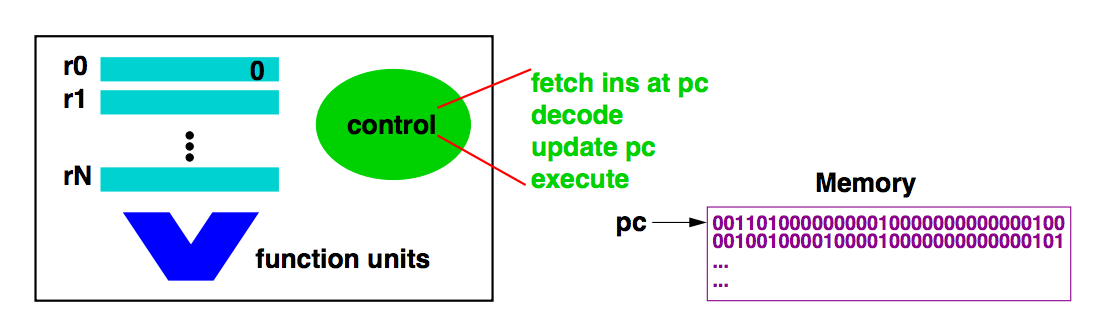
\includegraphics[scale=.7]{absComp}
  \caption{An Abstract Computer}
\end{figure}


\subsection{Instruction Set Architecture}
ISA is a contract between hardware and software: operands, data types, operations,
and encoding. It specifies the language that the CPU understands. Hardware can 
implement however as long as software cant distinguish. Software can use any syntax
as long as it translate to assembly. AKA everything is fair game people!

\subsubsection{Operands}
Data is either a constant (input value), in a register, or stored in memory. In 
the MSP 430 assembly, operands are usually 16-bit (possible to use 8-bit) and
distinguished with the \c{.b} vs \c{.w} extension. For example \c{mov.b} is to move a byte 
sized data where as \c{mov.w} is to move a word-sized data.

Arrays are implemented using memory because remember that all memory is essentially
part of the long spaghetti at the end of the day. 
\begin{C}
for (i=0; i<10; i++){
  x = x+ a[i];
}
//a:    the location in memory
//a[0]: the contents stored at location (a+0)
//a[1]: the contents stored at either (a+1) or (a+wordsize)
\end{C}

The location of operands in specified by the \emph{addressing mode}. The MSP 430
supports the following different addressing modes:
\begin{figure}[H]
  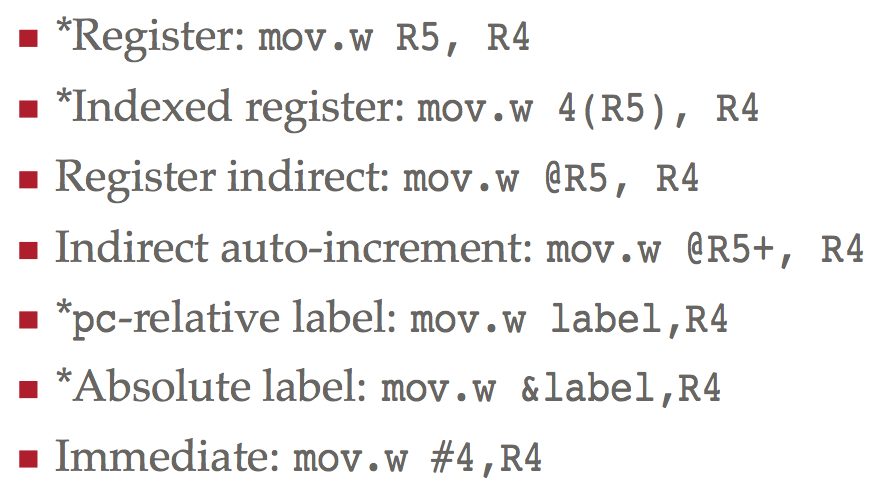
\includegraphics[scale=.5]{address}
\end{figure}

\subsubsection{Endianness}
Endianess comes into play when you want to break a large value (such as words) 
into several small ones (such as bytes). For implementation, there are two 
approaches to the order of the smaller parts. 
\begin{enumerate}
\item \textcolor{blue}{Big Endian}: Store the most significant byte in the smallest address
\item \textcolor{blue}{Little Endian}: Store the least significant byte in the 
  smallest address
\end{enumerate}
For example, if we wanted to store the value xFEED into a memory array, we could
use the following:
\begin{figure}[H]
  \centering
  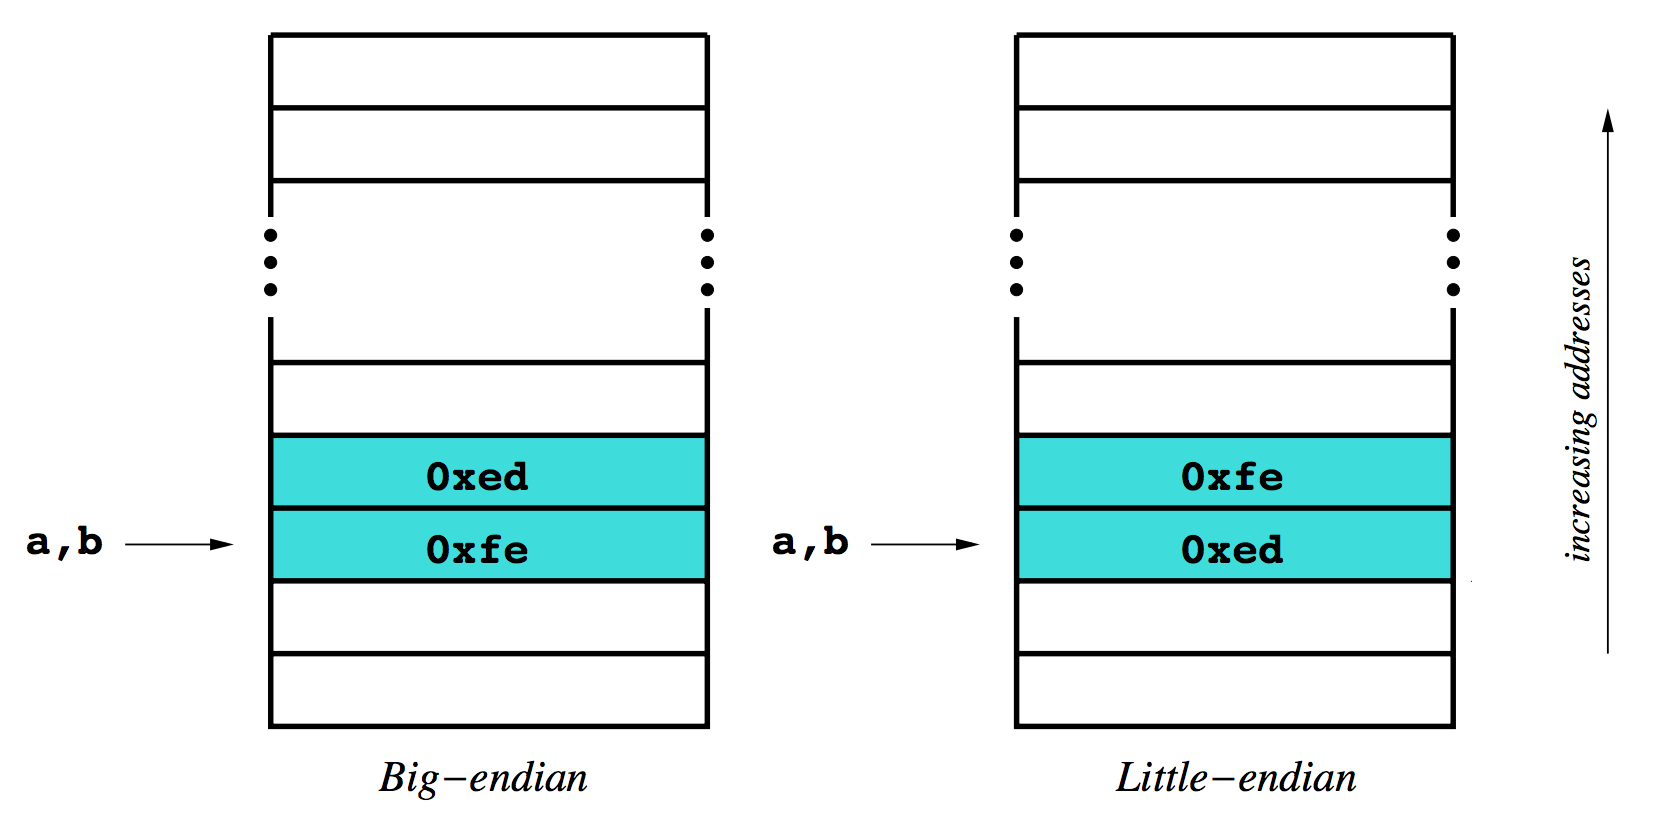
\includegraphics[scale=.4]{endian}
  \caption{Big Endian vs Little Endian}
\end{figure}

\section{Most Commonly Used Instructions}
\begin{figure}[H]
  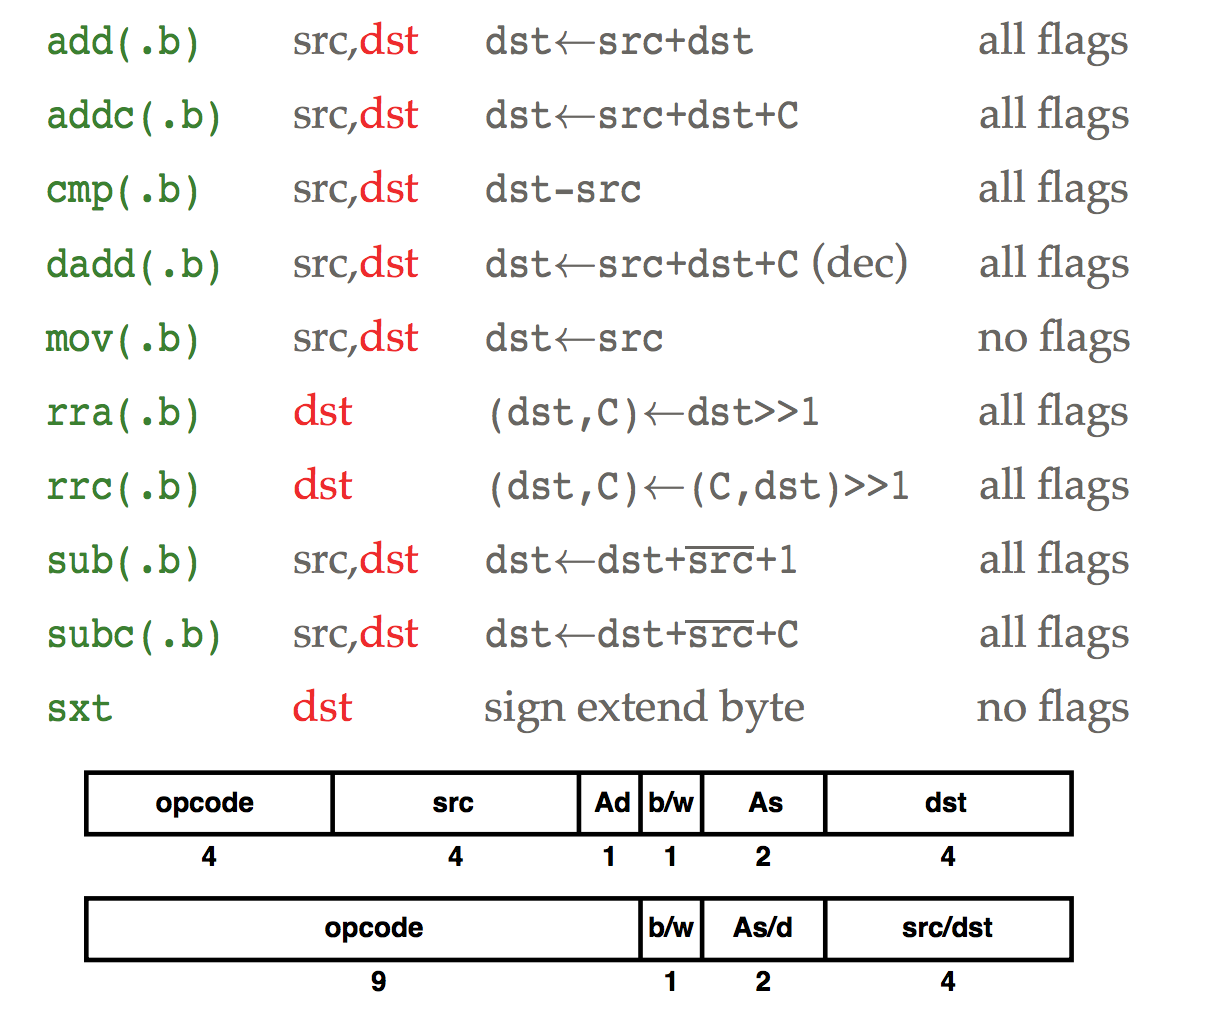
\includegraphics[scale=.6]{instructions}
\end{figure}


\section{Function Calls}
Functions are self contained modules of code that accomplish a specific task. 
In the MSP 430, there are general guidelines for implementing and using functions
that ensure that your data is saved and the you get the result you desire. 

\subsection{Stack}
The stack is a LIFO data structure that maintains the invariant that the last 
element inserted is the first element to be removed. This is an ideal structure
for function calls and especially for recursion. In the MSP 430, it looks something
like this:
\begin{figure}[H]
  \centering
  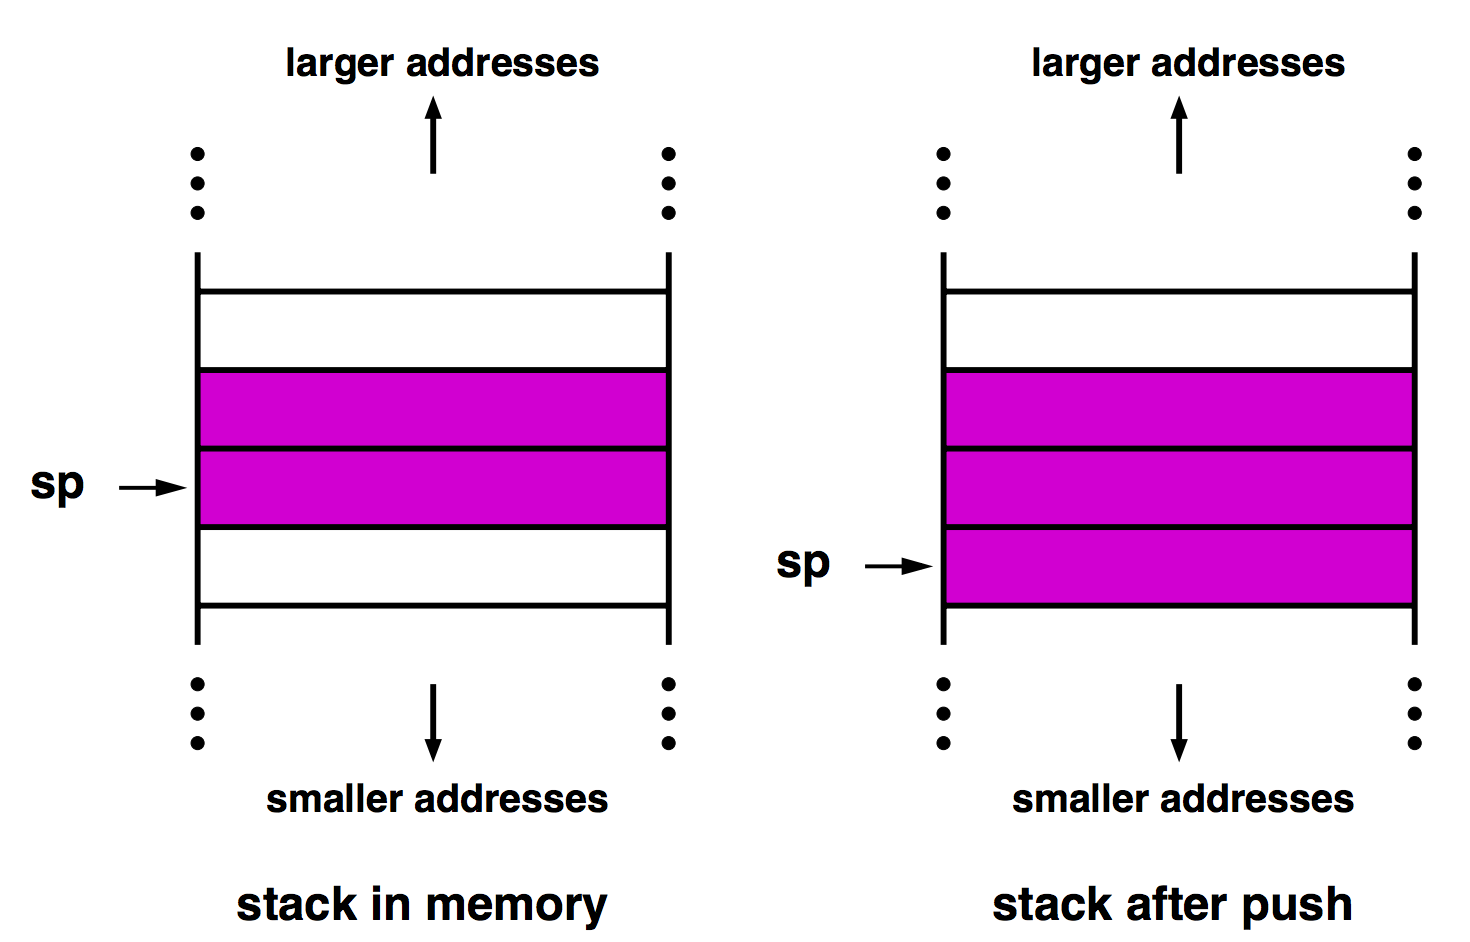
\includegraphics[scale=.4]{stack}
\end{figure}
To push to the stack we use the following command:
\begin{C}
  SP $\leftarrow$ SP-2
  @SP $\leftarrow$ src
\end{C}


\subsection{Order of Operations}
To properly implement a function call the following must occur:
\begin{enumerate}
  \item User pushes the caller saved registers onto the stack (R11-R15)
  \item User pushes any parameters onto the stack
  \item User uses the keyword \emph{call} to push the return addr onto the stack and jump
  to the function
  \item Function pushes callee saved registers onto stack (R4-R10)
  \item Function pushed any local variables on to the stack
  \item Function uses key word \emph{ret} to put the return addr into the PC and
    return to the caller. Its a pseudo instruction for mov.w @R1+, R0
\end{enumerate}
Therefore, the stack should look something like this:
\begin{table}[h]
\centering
\begin{tabular}{|c|}
  \hline
  R11  \\\hline
  R12-R15  \\\hline
  parameters  \\\hline
  ret address  \\\hline
  R4-R10  \\\hline
  local vars  \\\hline
\end{tabular}
\end{table}


\section{Assembling the Program}
\subsection{Assembler}
The assembler translates assembly language programs into machine code. It expands
pseudo operations, converts assembly to machine code, and outputs an 
\textcolor{blue}{object} file. Additionally, they keep track of where the jumps are,
and where references to labels are. There are two approaches to assemblers:
\begin{enumerate}
  \item Two-Pass: It allocates instruction and determines addresses on first pass
    and then assembles instructions knowing all labels.
  \item One-Pass: It assembles instructions putting zeros for unknown offsets and
    keeps track of unfinished instructions. When labels appear or at the end of
    oass one, it fills in unfinished instructions.
\end{enumerate}

\subsection{Linker}
The linker takes a collection of object files and libraries and generates an 
exectuable program.


\section{Input Output}
Three common ways to implement I/O are:
\begin{itemize}
  \item Special Instructions: They access the IO ports and the code is easy to 
    follow but you give up one opcode.
  \item Special Registers: Some registers are mapped to I/O ports but there are 
    only a limited number of registers anyways.
  \item Memory Mapped I/O: Certain memory address are linked to I/O ports and this
    saves new instructions since we can just use load and store (mov.w).
\end{itemize}

\subsection{Polling}
Polling is a common way to handle when to read input. 
Implementing polling-based input requires a loop that checks the value of a 
certain input register until its value is set by some hardware. Once we read
that the input flag is set, we can read and handle the input value. While the 
process is polling the input, the CPU cannot execute any other instructions. 
However, polling is very simple to implement and has very low overhead (3 instruction
loop) and can often be faster than interrupt driven input.

\subsection{Interrupts (async)}
In interrupt-based input, the CPU can execute other instructions and 
when the hardware of the input is set, it sends a signal to the CPU that there is
an input to be read. At this point, the current process is interrupted, its 
current PC and SR are pushed to the stack, the corresponding ISR is run, and 
finally the PC and SR are popped off so that the process can resume where it was
before. All registers become callee saved registers because it impossible to tell
when an interrupt is invoked. At the end we use to command \emph{reti}. The SR
has a bit that says if the CPU can be interrupted or not. Interrupt driven input
also requires more hardware support than polling. The asynchronous tag means that
we cannot at which instruction the interrupt occured. 

\subsection{Exceptions (sync)}
Exceptions are also handled through interrupts, however they are synchronous with
the execution of the program (divide by 0, page fault). For example a 
\emph{Page Fault} occurs when a page needed is in DISC so the ISR will bring the 
page into memory and then return back to the same instruction. The synchronous 
tag means that you can pin point exactly which instruction caused the exception
or trap.

\subsection{Service Routines (TRAPS)}
Service routines are responsible for reading and writing to the DISC\@. They 
encapsulate simple tasks for the user and invoke changes of privilege. For example,
when you boot up, you are in Super User mode so that you can define where SVC are
even located and then you change back to user mode.

\subsection{Daisy Chaining}
Daisy Chaining is a wiring scheme in which multiple devices are wired together 
in sequence. 
\begin{figure}[H]
  \centering
  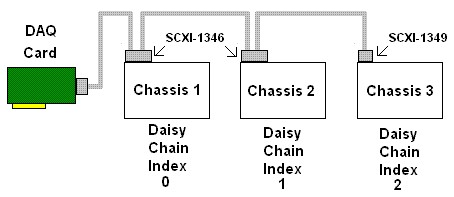
\includegraphics[scale=.8]{dchain}
\end{figure}

The closest connection has the highest priority. The problem is if there is any
electrical disconnect, all priorities will be lost.

\subsection{Interrupt Vector}
\begin{itemize}
  \item The Interrupt vector deallocates the system call `name' from actual ISR
    address.
  \item It allows flexibility in designing ISR code for a particular service
  \item Provides an organized `menu' of services
\end{itemize}


\section{Concurrency}
Concurrency is defined as running in parallel or operating at the same time. 
There are two types or resources involved here:

\begin{itemize}
  \item \textcolor{blue}{Shared Variables:} accessed by multiple processes and 
    their single read and write is atomic. Must be stored in global memory and not
    stack.
  \item \textcolor{blue}{Private Variables:} accessed by only 1 process and are
    not interfered
\end{itemize}

"Concerns in Mutual Exclusion:"
\begin{itemize}
  \item \textcolor{blue}{Safety:} At any moment, at most one process is in the 
  Critical Section
  \item \textcolor{blue}{Fairness:} If a process is continuously enabled, it will
    eventually get a chance to execute (Weak Fairness). Given many chances to
    execute, all processes will have a chance of running (Probablistic Fairness)
  \item \textcolor{blue}{Progress:} There is no Deadlock or Livelock
\end{itemize}

\subsection{Turn Approach}
\begin{figure}[H]
  \centering
  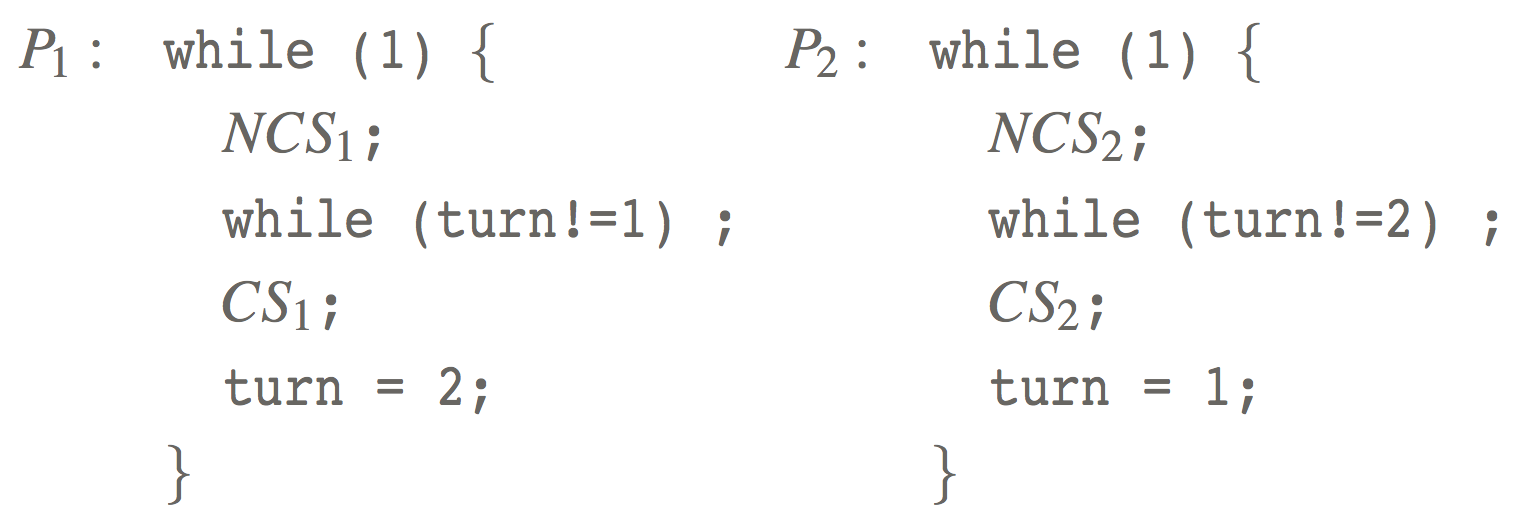
\includegraphics[scale=.4]{turn}
\end{figure}

\begin{itemize}
  \item Safety:    Yes - only one CS will execute at a time                 
  \item Fairness:  Yes  - probablistic fairness as long as there is progress but
    not weak fairness if crash in NCS
  \item Progress:  No - if you crash in one CS, no process can run          
\end{itemize}


\subsection{Dekker's Algorithm V1}
\begin{figure}[H]
  \centering
  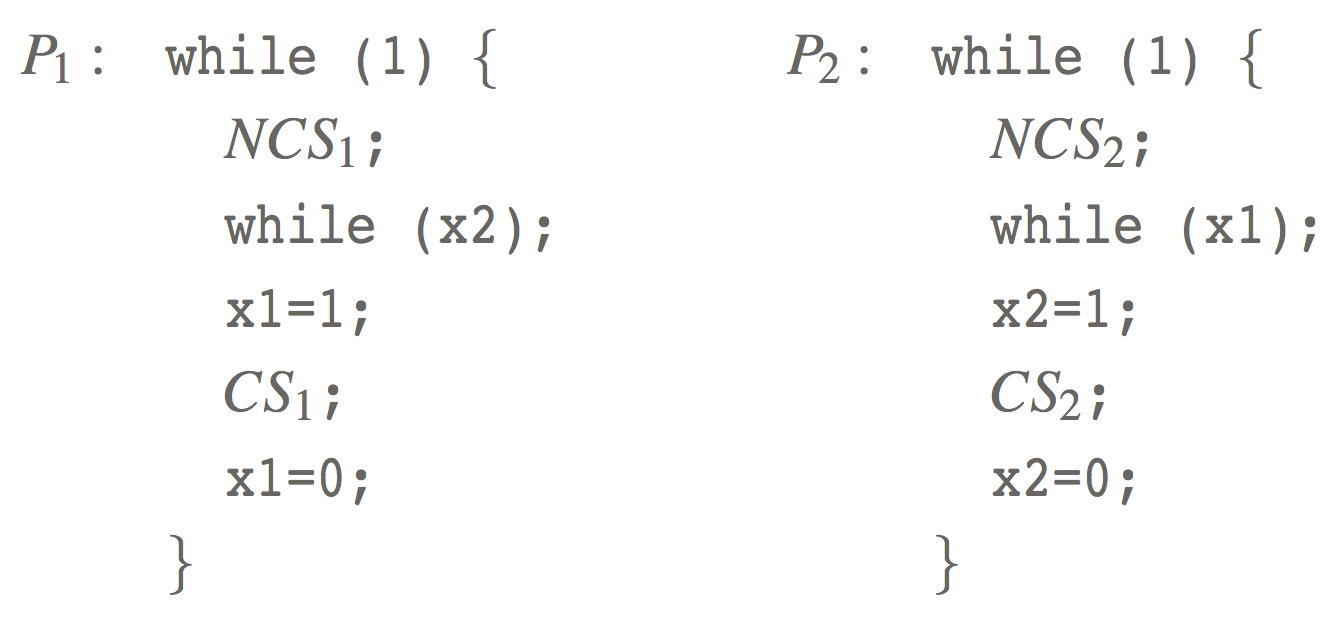
\includegraphics[scale=.4]{dekker1}
\end{figure}

\begin{itemize}
  \item Safety:    No - if x1 and x2 = 0, both can access CS at same time   
  \item Fairness:  Yes  - probablistic fairness, not always weak fairness 
  \item Progress:  Yes - if one CS crashes, other process can still run     
\end{itemize}

\subsection{Dekker's Algorithm V2}
\begin{figure}[H]
  \centering
  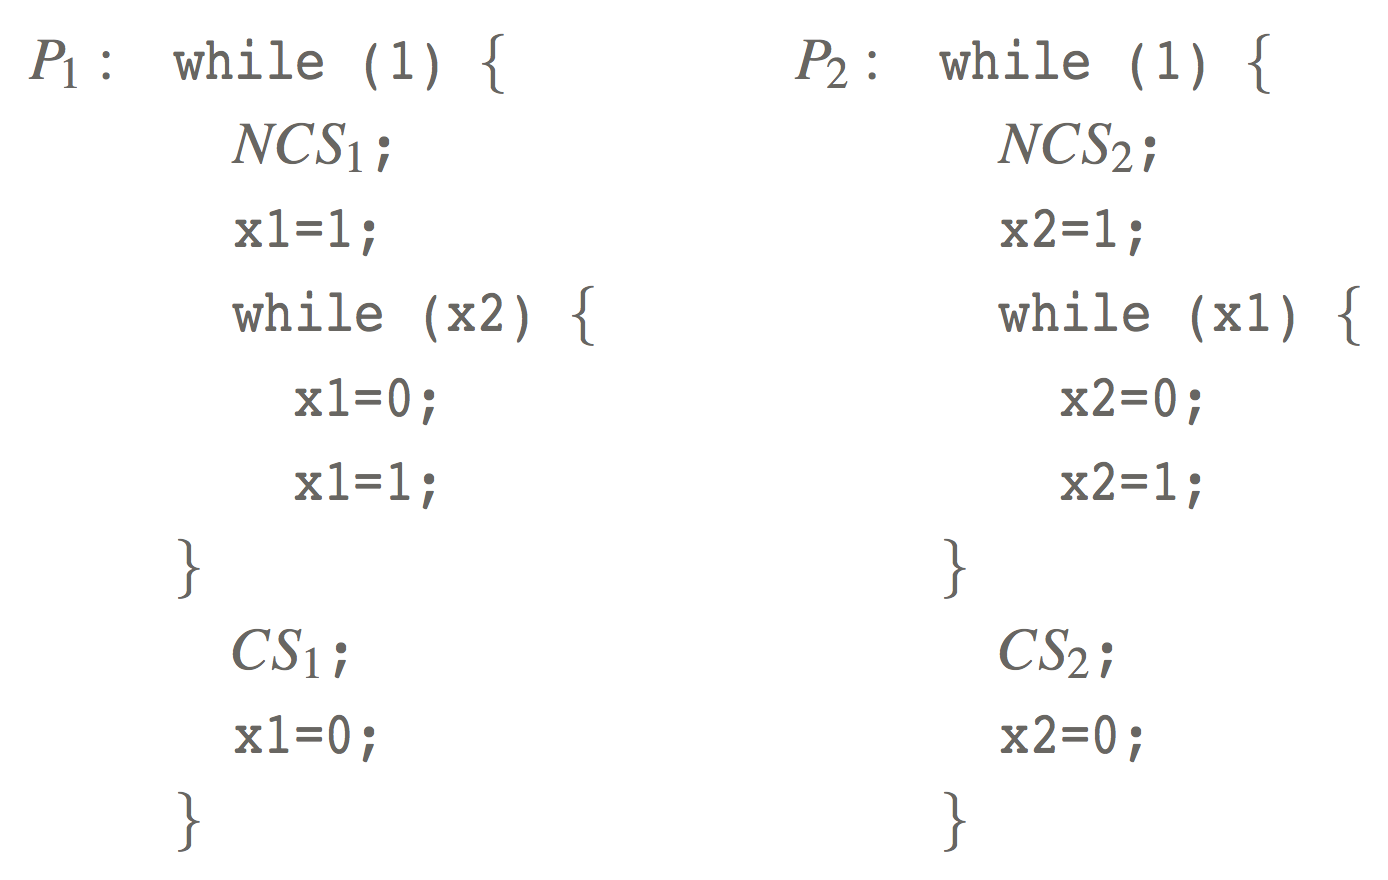
\includegraphics[scale=.4]{dekker2}
\end{figure}
                                                                        
\begin{itemize}
  \item Safety:    Yes - only one CS will execute at a time                 
  \item Fairness:  Yes - after one process completes CS, it yields to other and
    one NCS crash doesn't affect other
  \item Progress:  No - livelock can occur since x1 and x2 start as 1 and wait
    for each other to become 0. Classic `after you, no after you' problem                
\end{itemize}

\subsection{Dekker's Algorithm Final}
\begin{figure}[H]
  \centering
  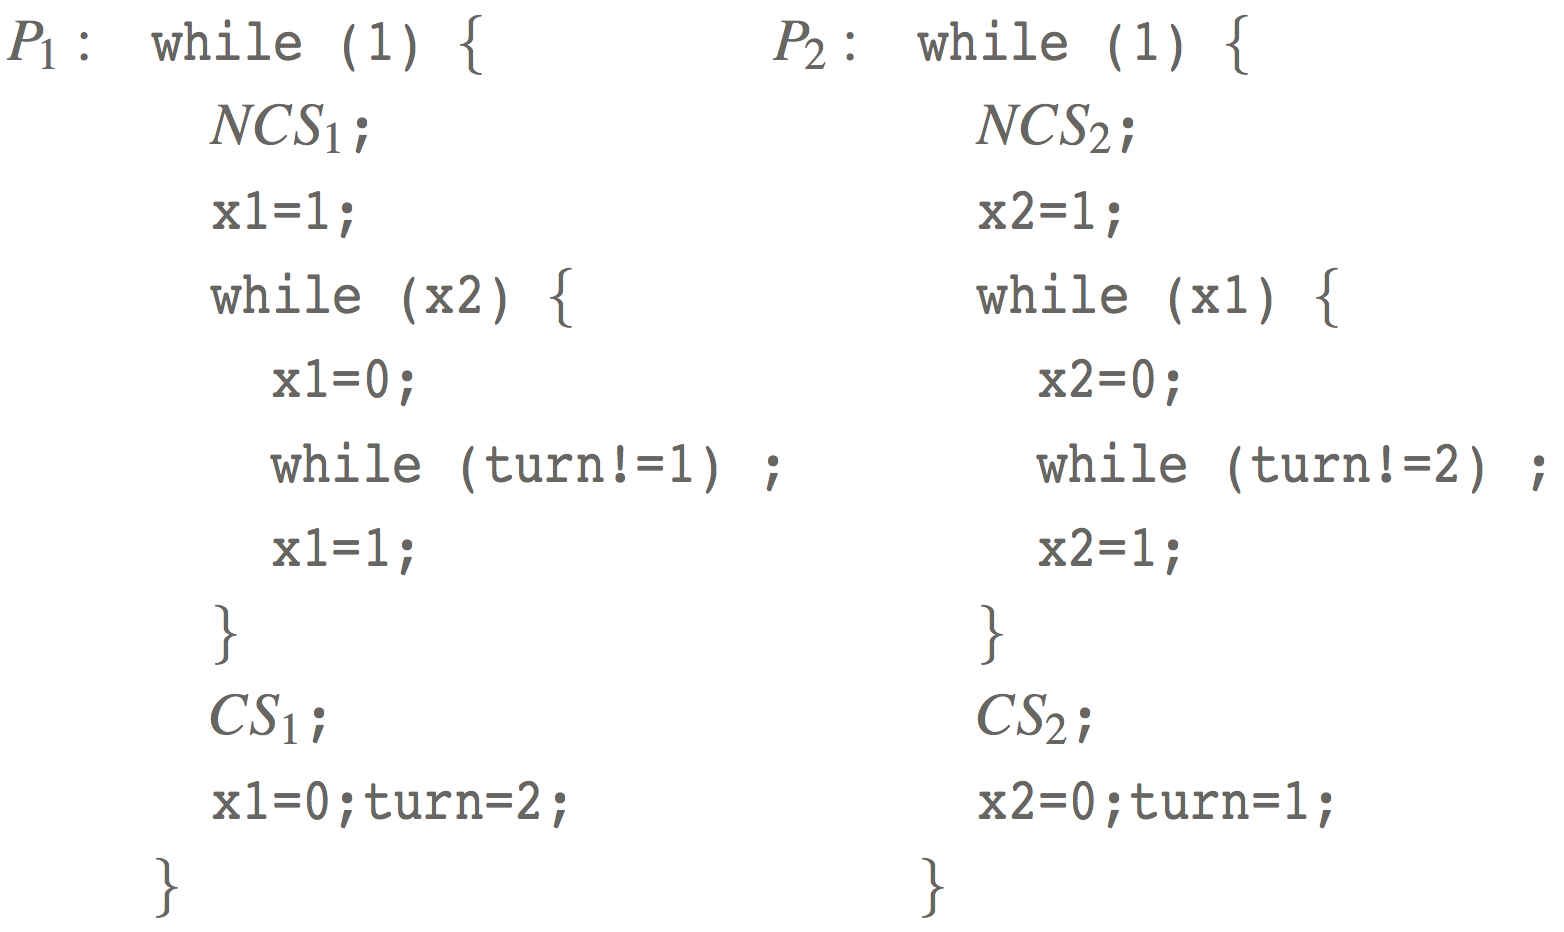
\includegraphics[scale=.4]{dekker3}
\end{figure}
                                                                        
\begin{itemize}
  \item Safety:    Yes - only one CS will execute at a time                 
  \item Fairness:  Yes - after one process completes CS, it yields to other and
    one NCS crash doesn't affect other 
  \item Progress:  Yes - with the use of turn, there is no chance of deadlock of livelock       
\end{itemize}


\section{Time Sharing - Implementing Concurrency}
A process can either be in the \emph{ready}, \emph{blocked}, or \emph{running}
state of a process contains:
\begin{itemize}
  \item Code: PC
  \item Data: Registers, memory variables (private and shared), stack
  \item State: Flags (SR) 
\end{itemize}

Each process contains its own stack space and has a SP. The rest of the state is
\emph{saved on the stack}. We maintain a queue of process in the ready state:
\begin{C}
struct process_state {
  uint sp;
  struct process_state *next;
};

typedef struct process_state process_t;
\end{C}

\begin{figure}[H]
  \centering
  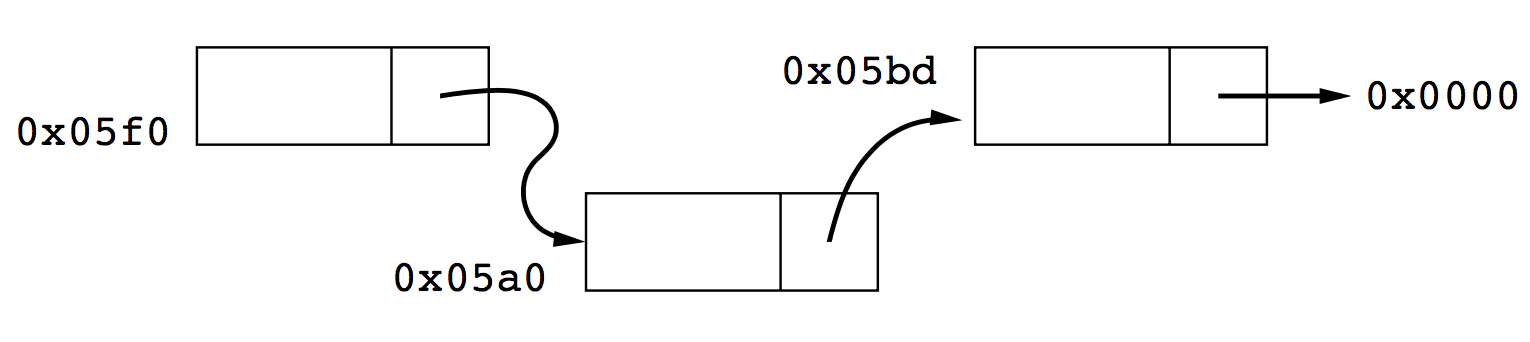
\includegraphics[scale=.4]{queue}
\end{figure}

\subsection{Context Switching}
Context Switching gives the illusiong of concurrency even though
all the processes are sharing one CPU.
Timer interrupts are used to stop process execution. In the handler, we pick up
the next ready process from the queue and update registers to correspond to that
process. The timer sets the quantum of the execution (\emph{time slice}). The
process of saving and restoring process state is called a context switch.
The procedure for switching processes using the Round Robin method:

\begin{enumerate}
  \item Push the PC, SR, and Registers of current process
  \item Update the SP of the current process 
  \item Grab the first process on the ready queue and make it the current process
  \item Restore the Registers, and use \emph{reti} to restore SR and PC
\end{enumerate}


\section{Locks}
A lock supports two basic - atomic operations:
\begin{itemize}
  \item lock(l)
  \item unlock(l)
\end{itemize}
Note this is simple an abstraction and locks can be implemented in many 
different ways.

\begin{figure}[H]
  \centering
  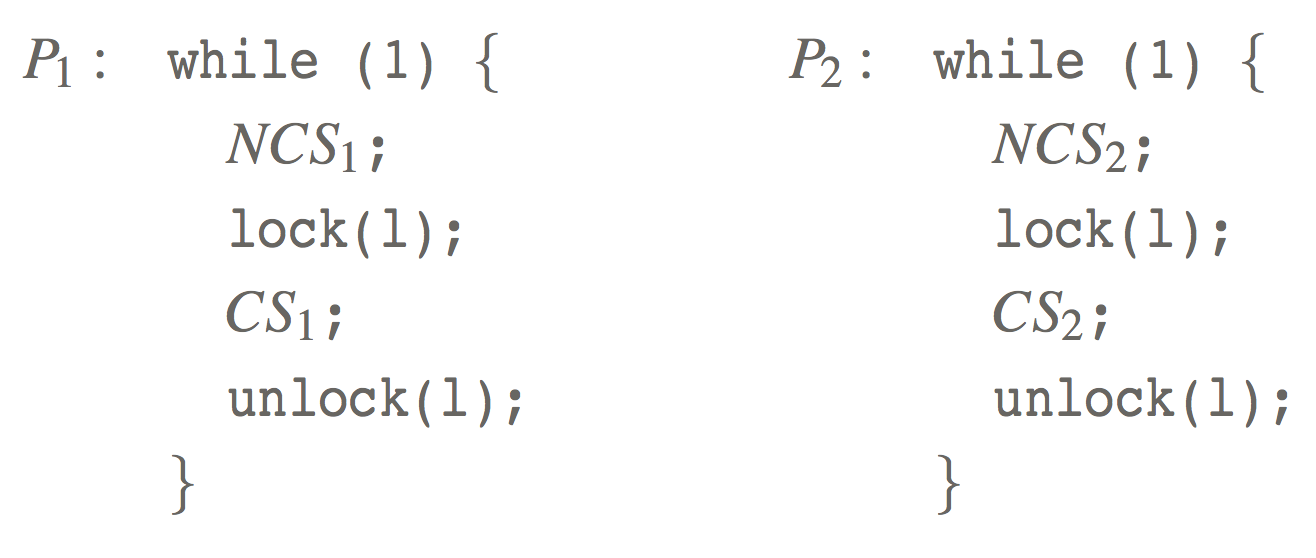
\includegraphics[scale=.4]{lock}
\end{figure}

\subsection{Test and Set}
Test and set instruction is an instruction used to write to a memory location 
and return its old value as a single atomic operation. It sets the Z flag 
according to the value read and sets the lock's value to 0. Below is how we
implement the lock() function seen above:
\begin{C}
Lock:   t&s &l
        jz Lock
\end{C} 
The advantage of this implementation is that it maintains an atomic instruction 
for RMW. It is very efficient and has low overhead. However, it is still a 
spin lock and 1 quantum is wasted just looping on a variable.
    
\subsection{Blocking Locks}
To avoid using a spin lock, we can use a blocking primitives. The basic idea behind
this is that the OS either gives the process access to the CS or it kicks it out
of the CPU (into blocked queue). However, there is more overhead here because we
have to switch to the SU mode. To implement this, we define a Trap routine to handle
the locking and this is useful because traps have access to OS functions as we are
in the SU mode. This is good for very small critical sections since we have to 
disable all interrupts. The pseudo code for this is as follows:
\begin{C}
GIE = 0; //OS does this internally, acts as a lock as all interrupts are disabled
if(l == 1){
  l = 0;
  return;
}
else{
  move process from ready queue to blocked queue;
}
\end{C}

\subsection{Readers and Writers Example}
There are two types of processes. Readers read a shared variable and Writers 
modify a shared variable. Reads and Writes are mutually exclusive. A simple 
approach uses two shared variables:
\begin{itemize}
  \item nw: number of writers
  \item nr: number of readers
\end{itemize}

\begin{figure}[H]
  \centering
  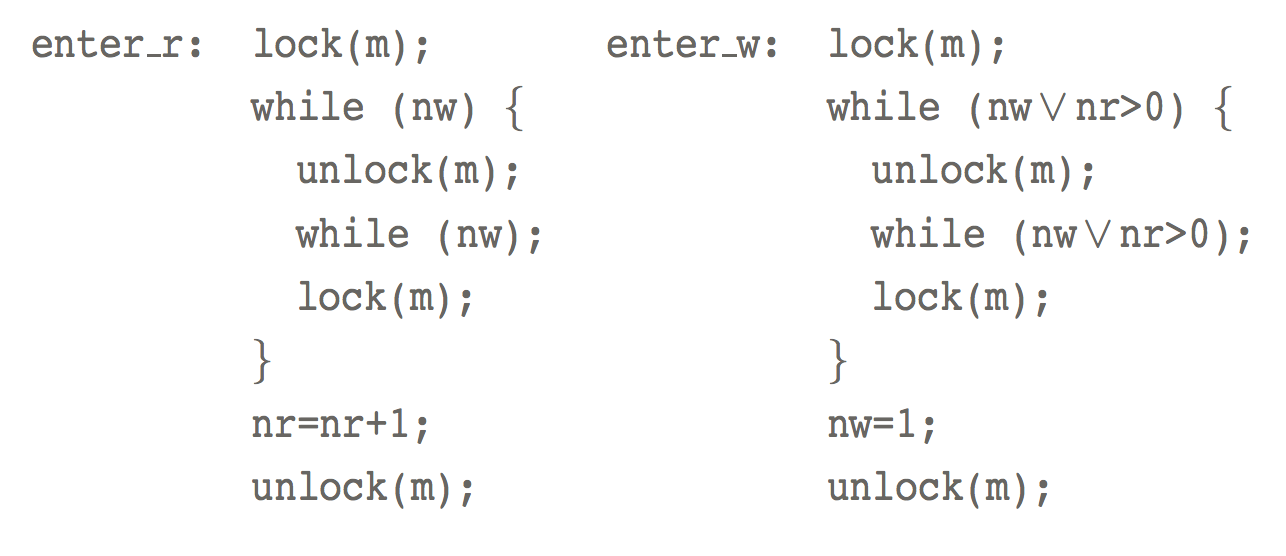
\includegraphics[scale=.6]{readwrite}
\end{figure}

Note: the locks in this case helps to implement a higher level construct of readers
and writers mutual exclusion and does not guarantee something for the Critical 
Section. The Critical Section is protected by \emph{nr} and \emph{nw} and these
two shared variables are protected by lock/unlock. We must also implement an exit()
function so that the readers eventually allow writers to write. Also, the while
loops in this example indicate that there is a spin lock which can be unwanted
and in the next section we will see another approach to this problem that avoids
the spin lock.


\section{Higher Level Constructs}
\subsection{Condition Variables}
A condition variable indicates an event and has no value. More precisely, one 
cannot store a value into nor retrieve a value from a condition variable. If a 
thread must wait for an event to occur, that thread waits on the corresponding 
condition variable. If another thread causes an event to occur, that thread 
simply signals the corresponding condition variable. Thus, a condition variable 
has a queue for those threads that are waiting the corresponding event to occur 
to wait on. Each condition variable has two basic operations: \emph{wait(l,c) and
signal(l,c)} where wait is a blocking operation.

\emph{wait(l,c):}
\begin{itemize}
  \item Waits for a condition to be signaled
  \item While it is waiting, the lock is released
  \item When we continue after the wait, the lock has been re-acquired
\end{itemize}

\emph{signal(l,c):}
\begin{itemize}
  \item Signals the condition
  \item It also releases the lock so that the next use of the release lock is a 
    process that was previously blocked on the wait
\end{itemize}

\emph{waiting(l,c):}
\begin{itemize}
  \item Returns true or false depending on whether or not there is a process
    blocked on the condition - you must hold the lock when this is executed.
\end{itemize}

\subsection{Another Look at Readers and Writers}
We can use Condition Variables to implement the read and write functions which 
eliminates spin locks.
\begin{figure}[H]
  \centering
  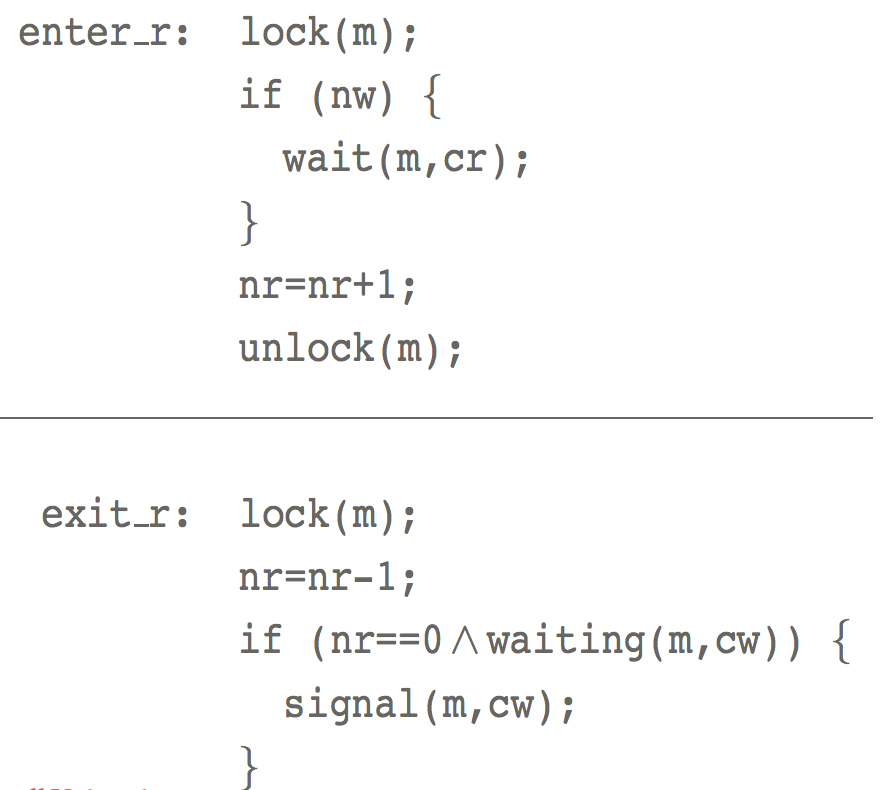
\includegraphics[scale=.5]{condition}
\end{figure}
However, when we don't to serialize readers, especially when there are no writers
present. To let ready readers execute, we can change \emph{enter\_r} so that there
are cascaded readers:
\begin{figure}[H]
  \centering
  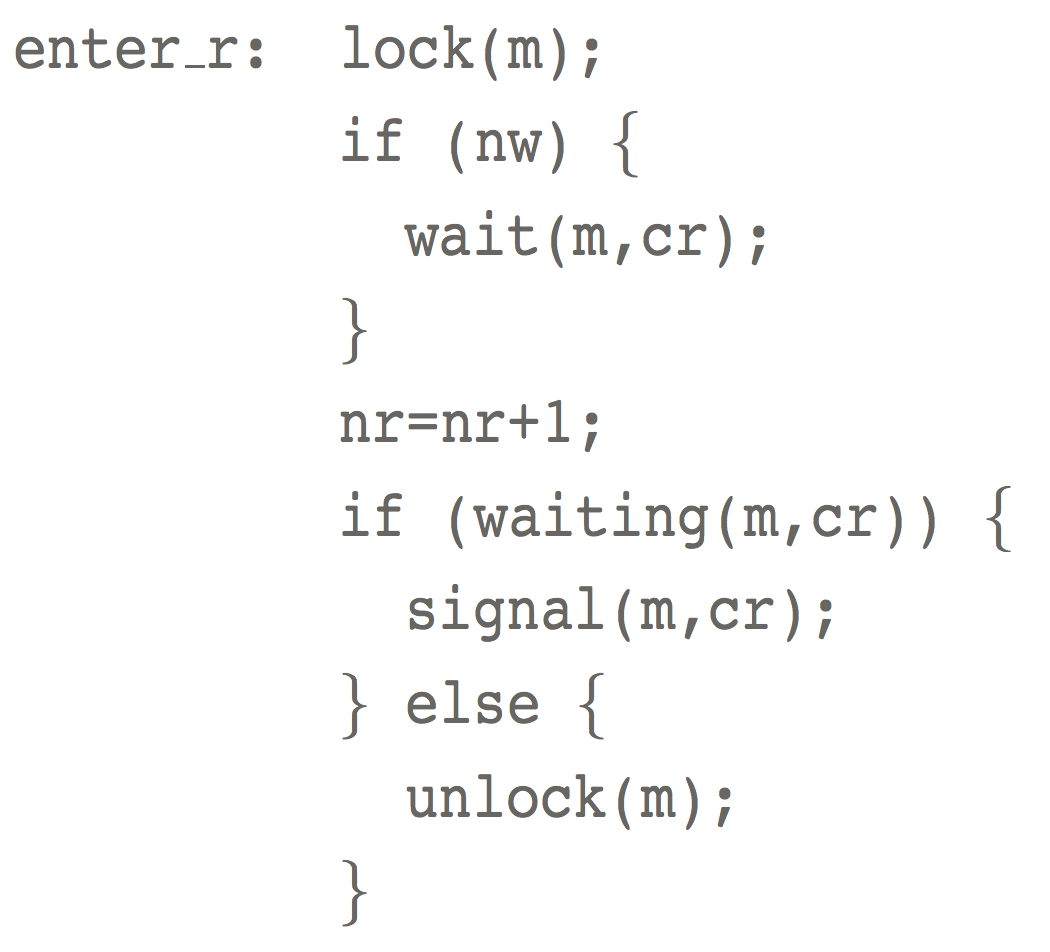
\includegraphics[scale=.4]{cascade}
\end{figure}

\subsection{Semaphores}
Think of semaphores as bouncers at a nightclub. There are a dedicated number of 
people that are allowed in the club at once. If the club is full no one is 
allowed to enter, but as soon as one person leaves another person might enter.
It's simply a way to limit the number of consumers for a specific resource. 

For example, a semaphore can be used to solve the Producers and Consumers problem
where we have processes that constantly try to write to a buffer and processes 
that constantly read from it.
\begin{figure}[H]
  \centering
  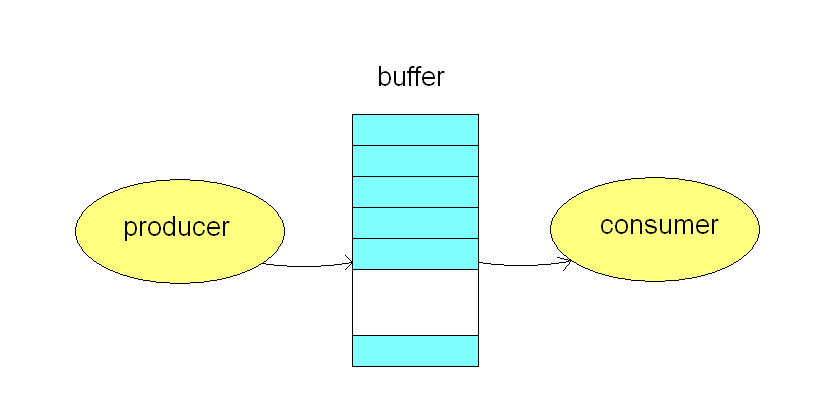
\includegraphics[scale=.45]{pcp}
\end{figure}

A very simple implementation of the following is shown below and we can see that 
there is spin lock that can be avoided:
\begin{C}
typedef struct{
    lock_t lock;
    int count;
}sem_t;

//Initilialze semaphor with count as the limit on the resource
void intit(sem_t *s, int c){
    lock(s->lock);
    s->count = c;
    unlock(s->lock);
}

//Write: Adds 1 to the count
void v(sem_t *s){
    lock(s->lock);
    s->count++;
    unlock(s->lock);
}

//Read: Waits until atleast 1 resource, and then decrements count
void p(sem_t *s){
    lock(s->lock);
    while(s->count < 1){
        unlock(s->lock);
        while(!s->count);
        lock(s->lock);
    }
    s->count--;
    unlock(s->lock);
}
\end{C}

To improve performance and avoid the spin lock,  we can use condition variables
so that other processes can utilize the CPU while a reader is waiting for at 
least one resource to be available. 
\begin{C}
void v(sem_t *s){
    lock(s->lock);
    s->count++;
    if(waiting(s->lock,s->count > 0)){
        signal(s->lock,s->count > 0);
    }
    unlock(s->lock);
}

void p(sem_t *s){
    lock(s->lock);
    if(!s->count){
        wait(s->lock, s->count > 0);
    }
    s->count--;
    unlock(s->lock);
}
\end{C}


\section{Event Driven Programming and Low Power Modes}
When the CPU is not doing anything, it goes to sleep $\rightarrow$ low power mode.
At this point, the processor waits to be awaken by an interrupt and this does 
require hardware support. The MSP430 has a 32 kHz crystal that drives all the low
power peripherals (sensors). This same crystal is fed into Digital Clock Signal
that produces a higher frequency that the CPU and high power peripherals use.

\begin{C}
while(1){
  wait for any interrupt;
  if(interrupt 0){
    operation 0;
  }else if(interrupt 1){
    operation 1;
  }...
}
\end{C}

The special codes to indicate low power modes are stored in the Status Register.
When the processor goes into low power mode, its SR is modified and it goes to 
sleep. When an interrupt occurs, the SR is pushed into the stack and a cleared SR
is given to the ISR to work with. When we return from the ISR, we don't want to
restore the SR because that would mean we go back to low power mode. Instead, the
ISR uses a hack where it goes to the stack and modifies the SR before \emph{reti}
is executed. 


\section{Extras}
\subsection{Peterson's Algorithm}
Peterson's algorithm is a concurrent programming algorithm for mutual exclusion
similar to Dekker's algo that allows 2 processes to share a resource without 
conflict. it uses two shared variables: \emph{flag} and \emph{turn}. 
A \emph{flag[n]} value of \emph{true} indicates that the process n wants to enter
the CS. Entrance to the CS is granted for the process P0 if P1 does not want to 
enter its critical section or it P1 has given priority to P0 by setting \emph{turn}
to 0.

\begin{C}
bool flag[0]   = false;
bool flag[1]   = false;
int turn;

P0:      flag[0] = true;
P0_gate: turn = 1;
         while (flag[1] && turn == 1)
         {
             // busy wait
         }
         // critical section
         ...
         // end of critical section
         flag[0] = false;

P1:      flag[1] = true;
P1_gate: turn = 0;
         while (flag[0] && turn == 0)
         {
             // busy wait
         }
         // critical section
         ...
         // end of critical section
         flag[1] = false;
\end{C}

\begin{itemize}
  \item Safety: Yes - P0 and P1 can never be in the critical section at the same time:
    If P0 is in its critical section, then flag[0] is true. In addition, either 
    flag[1] is false (meaning P1 has left its critical section), or turn is 0 
    (meaning P1 is just now trying to enter the critical section, but graciously
    waiting), or P1 is at label P1\_gate (trying to enter its critical section,
    after setting flag[1] to true but before setting turn to 0 and busy waiting) 
  \item Fairness: Yes - there is weak fairness, both processes will eventually
    get CS and if you crash in NCS, the other process can still execute
  \item Progress: Yes - A process cannot immediately re-enter the critical 
    section if the other process has set its flag to say that it would like to 
    enter its critical section and there is no chance for livelock or deadlock.
\end{itemize}


\end{document}

%SEE BAKER'S ALORITHM

